%\newcommand{\notatki}{1}
\documentclass{sa}
\usepackage{array} %dla poziomego wyrownania (m) w tabeli
\usepackage{soul}
\usepackage{bm}

\newcommand{\ang}[1]{(ang. \emph{#1})}
\renewcommand{\vec}[1]{\ensuremath\boldsymbol{#1}}
\newcommand{\grad}{\ensuremath\nabla}
\let\avg\overline

\usetikzlibrary{datavisualization}
\usetikzlibrary{datavisualization.formats.functions}

\usepackage{hyperref}
\graphicspath{{07_rl/}}
\subtitle{Uczenie ze wzmocnieniem}
\begin{document}
\begin{frame}
\titlepage
\end{frame}

\begin{frame}{Uczenie ze wzmocnieniem \ang{Reinforcement learning}}
\begin{description}
\item[dane] \alert{Środowisko}, w którym można wykonywać pewne \alert{akcje}, które są \alert{nagradzane} lub \alert{karane}, ale nie koniecznie od razu.
\pause
\item[zadanie] Znaleźć \alert{politykę}, która w długiej perspektywie czasowej maksymalizuje nagrody.
\end{description}
\end{frame}

\begin{frame}{Przykładowe środowiska, kary i nagrody}
\centering
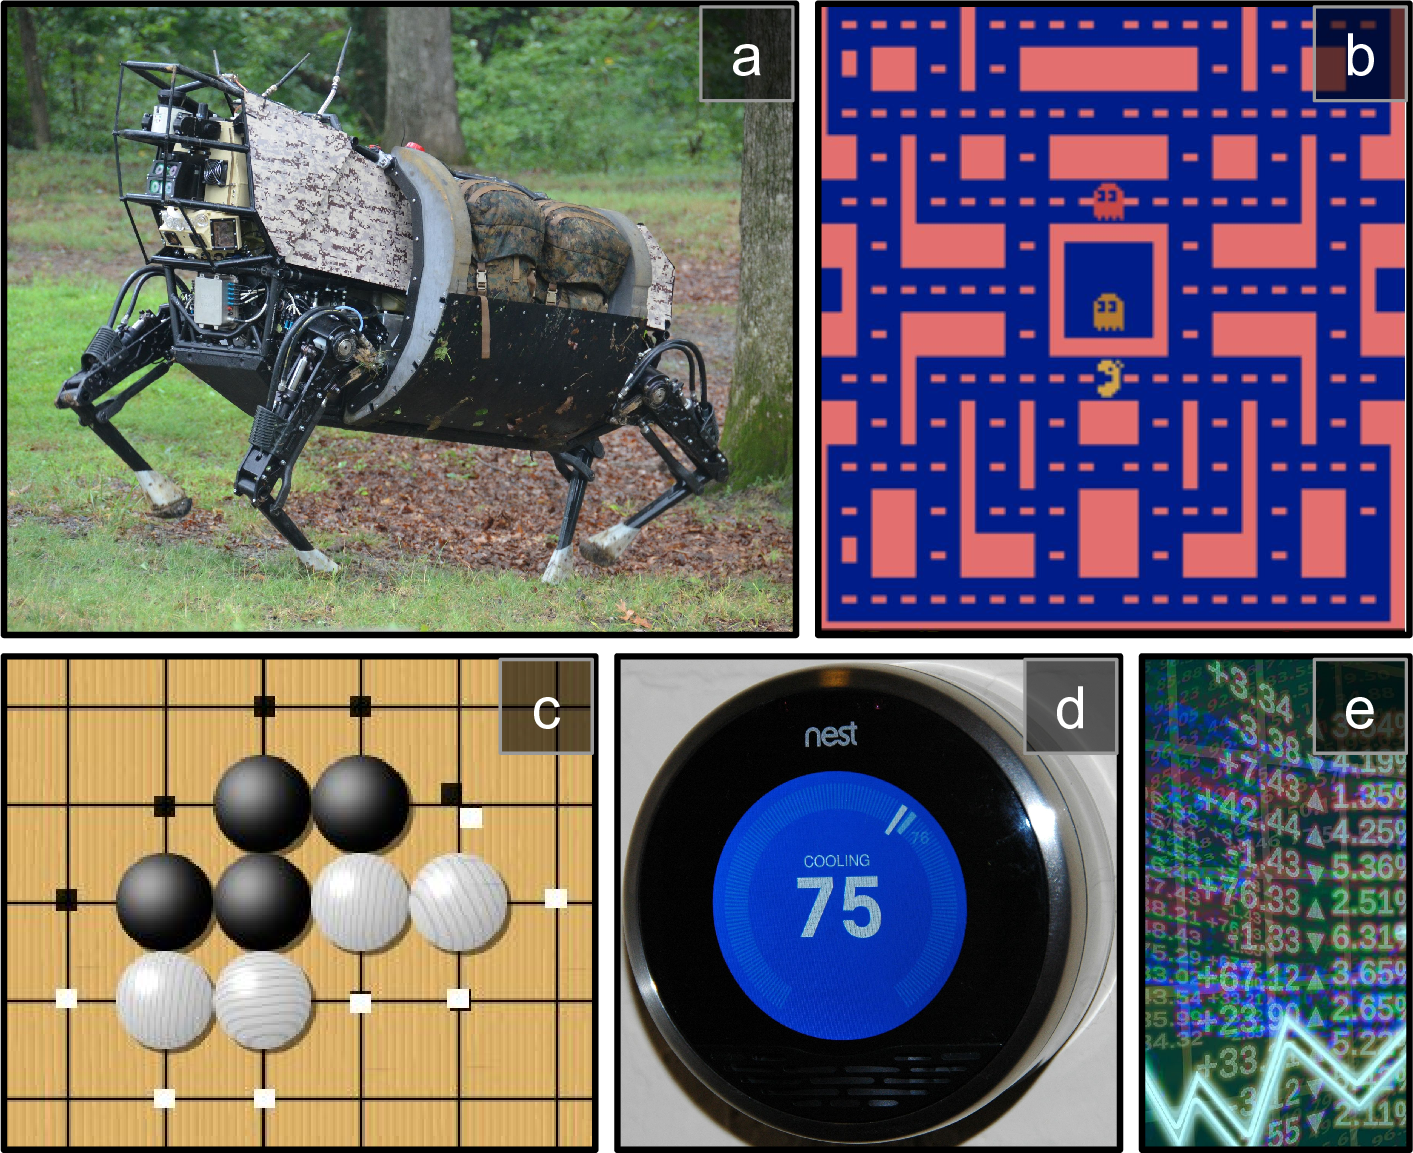
\includegraphics[width=.75\textwidth]{mlst_1601.png}
{\vfill\footnotesize A. Géron, \emph{Hands-On Machine Learning with Scikit-Learn and TensorFlow} 2017}
\end{frame}

\begin{frame}{Polityka \ang{policy}}
\begin{itemize}
\item<+-> Dowolny algorytm, który mówi, jaką akcję wykonać.
\item<+-> Polityka \alert{stochastyczna} -- jeżeli jest w tym aspekt losowości.
\end{itemize}
\end{frame}

\begin{frame}{Przykład polityki}
\centering
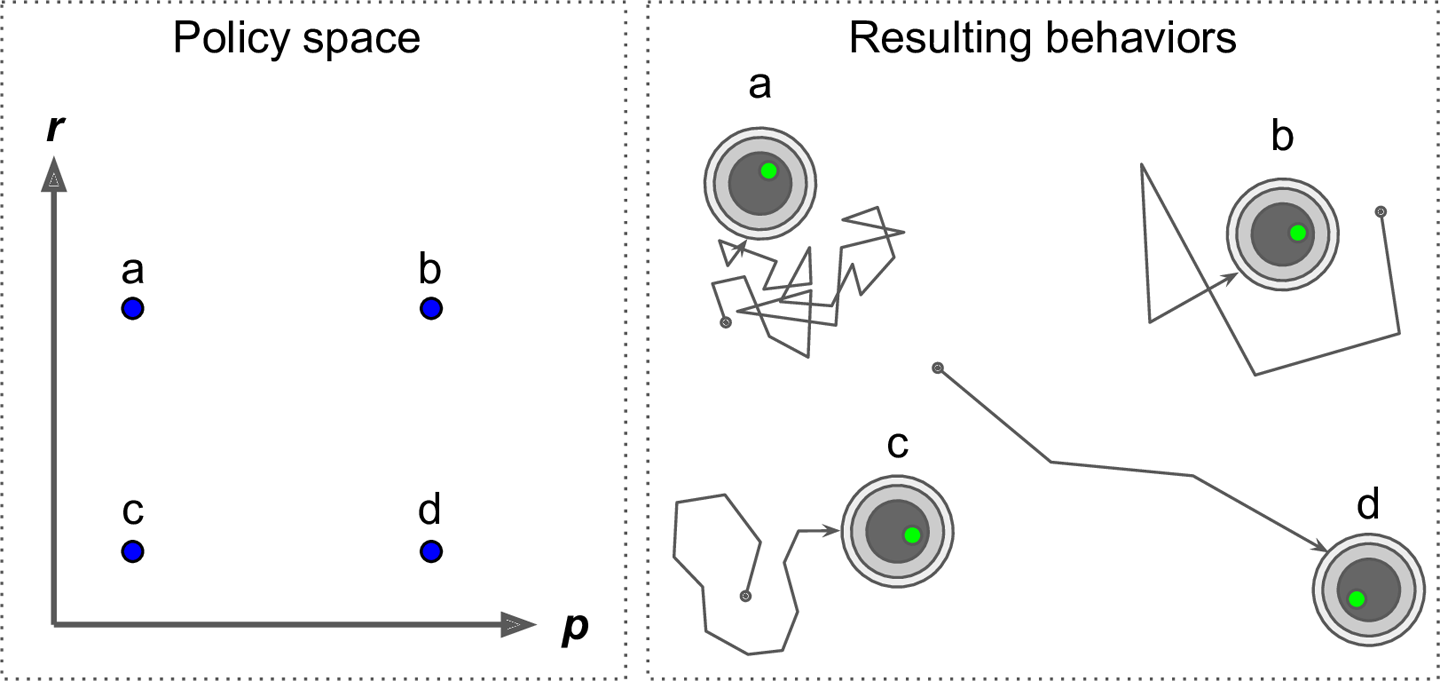
\includegraphics[width=\textwidth]{mlst_1603.png}
{\vfill\footnotesize A. Géron, \emph{Hands-On Machine Learning with Scikit-Learn and TensorFlow} 2017}
\note<1>{$p$ to prawdopodobieństwo jechania prosto (czyli $1-p$ to pr. zakrętu), a $r$ to kąt zakrętu}
\end{frame}

\begin{frame}{Toy example: cart pole}
\centering
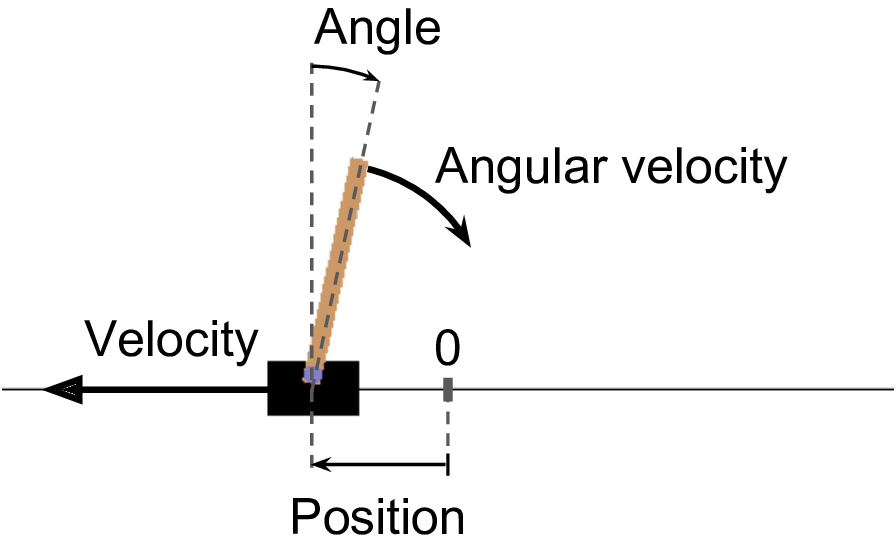
\includegraphics[width=.8\textwidth]{mlst_1604.png}\\
\pause
\alert{Cel:} wózek na środku, wahadło w pionie \\
\pause
\alert{Akcje:} siła 1 w lewo, siła 1 w prawo
{\vfill\footnotesize A. Géron, \emph{Hands-On Machine Learning with Scikit-Learn and TensorFlow} 2017}
\end{frame}

\begin{frame}{Polityka za pomocą sieci neuronowej}
\centering
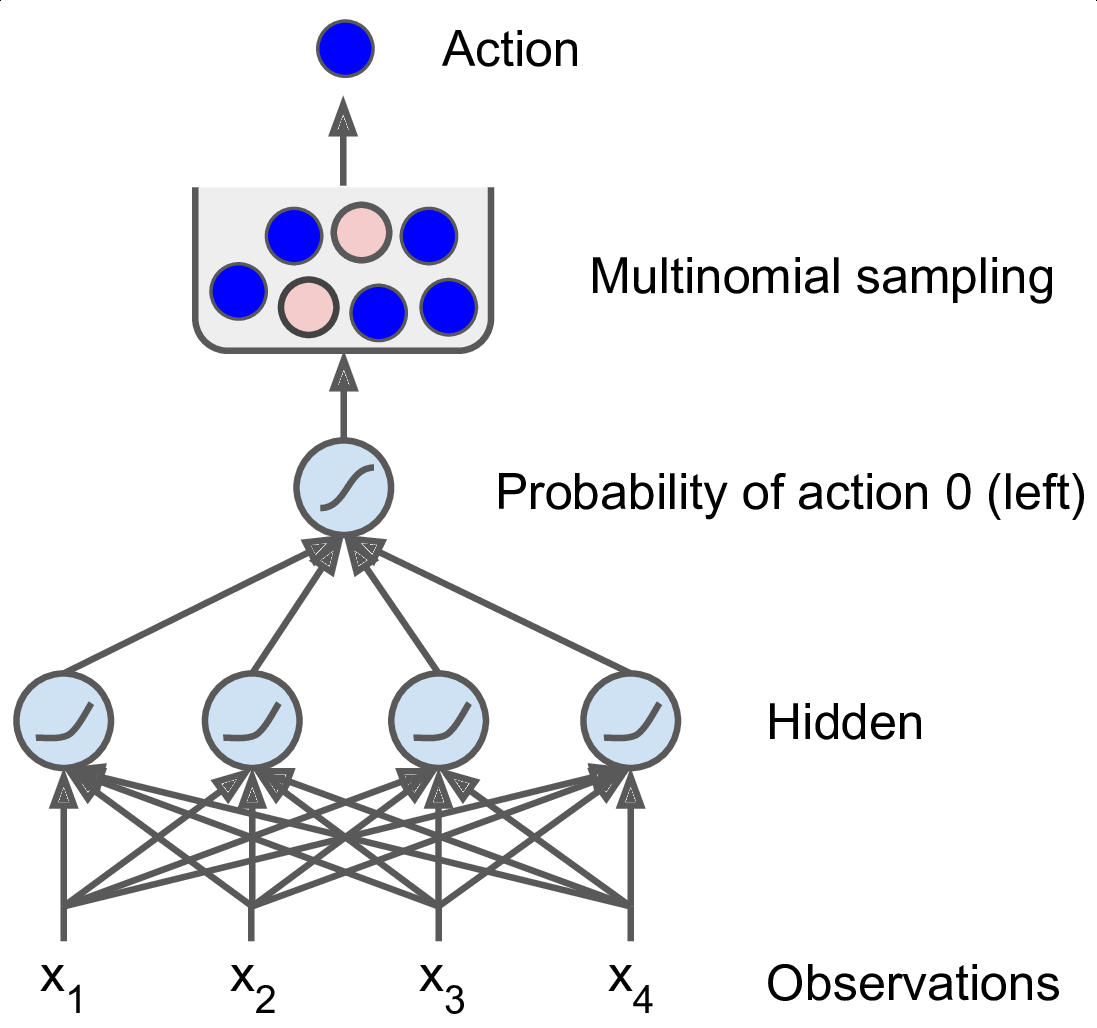
\includegraphics[width=.6\textwidth]{mlst_1605.png}
{\vfill\footnotesize A. Géron, \emph{Hands-On Machine Learning with Scikit-Learn and TensorFlow} 2017}
\note<1>{Losowanie, żeby zapewnić eksplorację}
\end{frame}

\begin{frame}{Obliczanie nagrody}
\centering
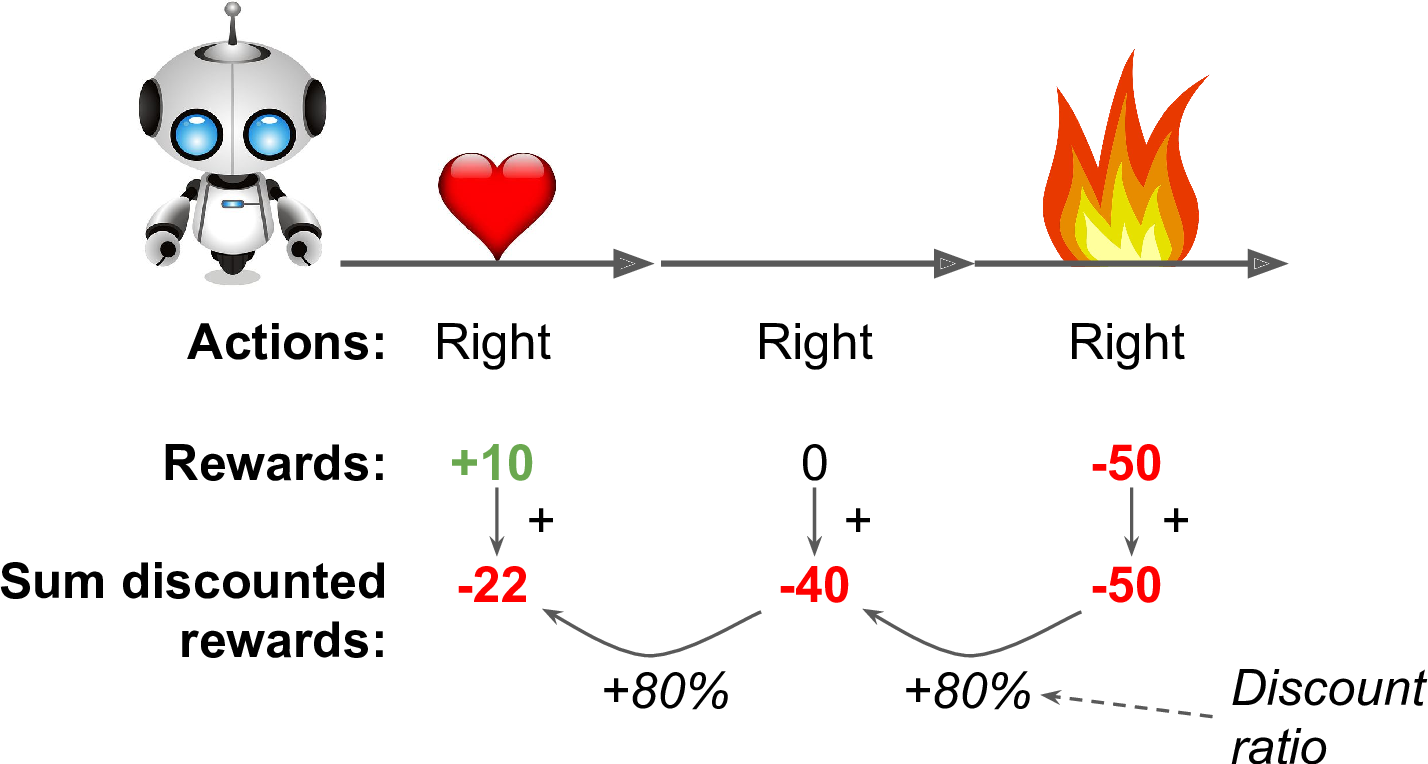
\includegraphics[width=\textwidth]{mlst_1606.png}
{\vfill\footnotesize A. Géron, \emph{Hands-On Machine Learning with Scikit-Learn and TensorFlow} 2017}
\end{frame}

\begin{frame}{Policy gradient: REINFORCE}
\begin{enumerate}
\item<+-> Zagraj w grę kilkukrotnie, w każdym kroku oblicz gradient wzmacniający wybraną akcję (tj. tak, jakby wybrana akcja była najlepsza możliwa)
\item<+-> Oblicz nagrodę każdej akcji:
\begin{enumerate}
\item<+-> Uwzględnij przyszłe nagrody przez \emph{discount ratio}
\item<+-> Dokonaj normalizacji odejmując średnią i dzieląc przez odchylenie standardowe (po wszystkich zdyskontowanych nagrodach)
\end{enumerate}
\item<+-> Pomnóż gradienty przez odpowiadające im znormalizowane nagrody
\item<+-> Uśrednij i zaaplikuj gradienty
\end{enumerate}
\end{frame}

\begin{frame}{Proces decyzyjny Markowa}
\centering
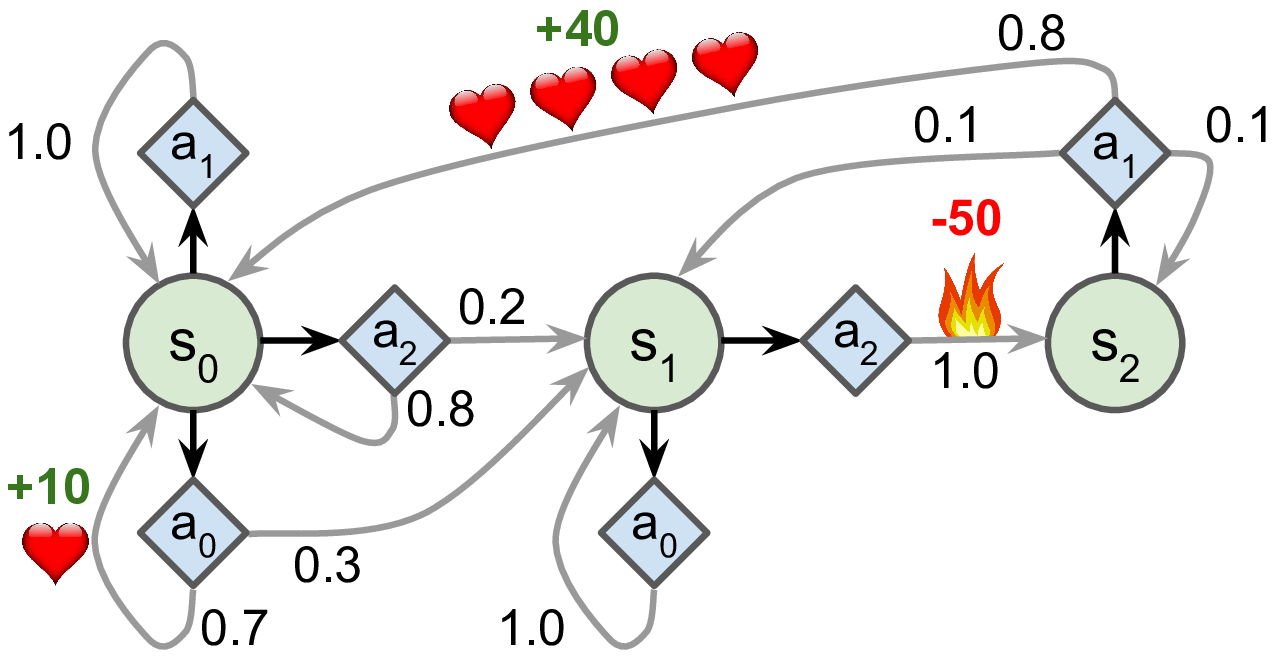
\includegraphics[width=\textwidth]{mlst_1608.png}
{\vfill\footnotesize A. Géron, \emph{Hands-On Machine Learning with Scikit-Learn and TensorFlow} 2017}
\end{frame}

\begin{frame}{Q-Value iteration}
\begin{itemize}
\item $Q_k(s,a)$ wartość akcji $a$ w stanie $s$ w kroku $k$
\item $T(s, a, s')$ prawdopodobieństwo przejścia $s\to s'$ przy akcji $a$
\item $R(s, a, s')$ nagroda za przejście $s\to s'$ przy akcji $a$
\item $\gamma$ discount ration
\end{itemize}
\pause
\[ Q_{k+1}(s,a) \leftarrow \sum_{s'} T(s, a, s')\left[R(s,a,s') + \gamma \max_{a'} Q_k(s',a') \right] \]
\pause
\[ \pi^{*}(s) = \arg\max_{a} Q_{\infty}(a) \]
\pause
\alert{Eleganckie, ale kompletnie niepraktyczne}
\note<.>
{
$T$ i $R$ są nieznane, a do tego liczba możliwych stanów zwykle będzie gigantyczna, więc nie da się wykonać odpowiednich obliczeń.
}
\end{frame}

\begin{frame}{Q-Learning}
\[ Q_{k+1}(s,a) \leftarrow (1-\alpha) Q_k(s,a) + \alpha \left(r + \gamma \max_{a'} Q_k(s', a')\right) \]
\note{$\alpha$ to prędkość uczenia. Wciąż niepraktyczne, bo większości par $(s,a)$ nigdy nie odwiedzimy.}
\end{frame}

\begin{frame}{Approximate Q-Learning}
Funkcja celu w uczeniu:
\[ y(s, a) = r + \gamma\max_{a'} Q(s', a') \]
\begin{itemize}
\item $Q(s,a)$ to funkcja, której się uczymy (realizowana np. przez sieć neuronową)
\item $s'$ to stan do którego przejdziemy po wykonaniu $a$ w $s$
\end{itemize}
\end{frame}

\begin{frame}{DeepMind Deep Q-Learning}
\begin{itemize}
\item<+-> to samo co przed chwilą (prawie)
\item<+-> replay memory
\item<+-> dwie sieci: online i target
\begin{itemize}
\item<+-> online się uczy
\item<+-> target oblicza $Q(s',a')$
\item<+-> okresowo kopiujemy online do target
\end{itemize}
\end{itemize}
\end{frame}

\end{document}